\section{Event buffer}\label{ch:eventBuffer}
The event buffer IPBus slave has four registers.
Writing to \verb|EventFifoCSR| will reset the \gls{fifo}. Reading from either of the register will put their data on the IPBus data line.\\
Reading from \verb|EventFifoCSR| returns the following:
\begin{itemize}
  \item bit 0: \gls{fifo} empty flag
  \item bit 1: \gls{fifo} almost empty flag
  \item bit 2: \gls{fifo} almost full flag
  \item bit 3: \gls{fifo} full flag
  \item bit 4: \gls{fifo} programmable full flag
  \item other bits: 0
\end{itemize}


The status register (SerdesRst) is as follows:
\begin{itemize}
  \item bit 0: reset the ISERDES
  \item bit 1: reset the trigger counters
  \item bit 2: calibrate IDELAY: This seems to be disconnected at the moment.
  \item bit 3: fixed to 0
  \item bit 4, 5: status of \verb|thresholdDeserializer(Input0)|. When the IDELAY modules (prompt, delayed) have reached the correct delay, these two bits should read 00.
  \item bit 6, 7: status of \verb|thresholdDeserializer(Input1)|
  \item bit 8, 9: status of \verb|thresholdDeserializer(Input2)|
  \item bit 10, 11: status of \verb|thresholdDeserializer(Input3)|
  \item bit 12, 13: status of \verb|thresholdDeserializer(Input4)|
  \item bit 14, 15: status of \verb|thresholdDeserializer(Input5)|
  \item bit 16, 19: fixed to 0
  \item bit 20: \verb|s_deserialized_threshold_data(Input0)(7)|
  \item bit 21: \verb|s_deserialized_threshold_data(Input1)(7)|
  \item bit 22: \verb|s_deserialized_threshold_data(Input2)(7)|
  \item bit 23: \verb|s_deserialized_threshold_data(Input3)(7)|
  \item bit 24: \verb|s_deserialized_threshold_data(Input4)(7)|
  \item bit 25: \verb|s_deserialized_threshold_data(Input5)(7)|
  \end{itemize}

9 bits are used to determine trigger edges. 8 are from the deserializers, 1 is added as the LSB and is the MSB from the previous word.

\begin{figure}
  \centering
  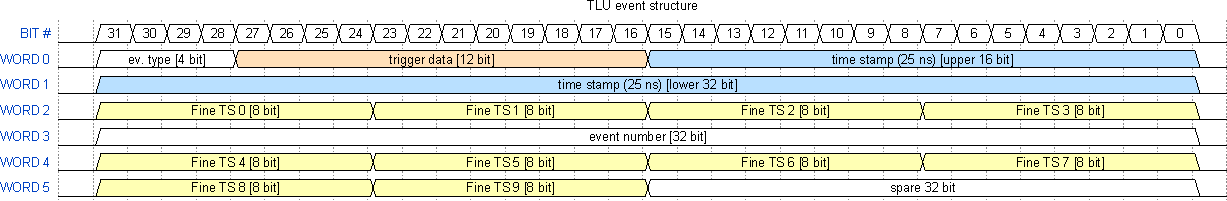
\includegraphics[width=.95\textwidth]{./Images/fifo_words.pdf}
  \caption{Event structure}
  \label{fig:fifo_event}
\end{figure}
